\documentclass{article}

\usepackage{fancyhdr} % Required for custom headers
\usepackage{lastpage} % Required to determine the last page for the footer
\usepackage{extramarks} % Required for headers and footers
\usepackage[usenames,dvipsnames]{color} % Required for custom colors
\usepackage{graphicx} % Required to insert images
\usepackage{listings} % Required for insertion of code
\usepackage{courier} % Required for the courier font
\usepackage{caption}
\usepackage{multirow, float}
\usepackage{subcaption}
\usepackage{graphicx}


\renewcommand{\_}{\char`_}
\renewcommand{\tt}{\lstinline}

% Margins
\topmargin=-0.45in
\evensidemargin=0in
\oddsidemargin=0in
\textwidth=6.5in
\textheight=9.0in
\headsep=0.25in

\linespread{1.1} % Line spacing


% Set up the header and footer
\pagestyle{fancy}
\lhead{Group 24} % Top left header
\chead{Corsair} % Top center head
\rhead{\firstxmark} % Top right header
\lfoot{\lastxmark} % Bottom left footer
\rfoot{Page\ \thepage\ of\ \protect\pageref{LastPage}} % Bottom right footer
\renewcommand\headrulewidth{0.4pt} % Size of the header rule
\renewcommand\footrulewidth{0.4pt} % Size of the footer rule

\setlength\parindent{0pt} % Removes all indentation from paragraphs

%----------------------------------------------------------------------------------------
%	TITLE PAGE
%----------------------------------------------------------------------------------------

\title{
\vspace{2in}
\textmd{\textbf{Project Documentation}}\\
\normalsize\vspace{0.1in}\small{Due\ on\ Monday,\ June\ 6,\ 2016}\\
\vspace{0.1in}\large{\textbf{WebApps Group 24: Corsair}}
\vspace{3in}
}

\author{Mery Noa Bendahan \\ Ignacio Navarro \\ Dan Slocombe \\ Tom Griggs \\ Jaime Rodriguez}
\date{}

%----------------------------------------------------------------------------------------

\begin{document}

\maketitle
\newpage


\section{Leaflet}
\clearpage
\section{System Architecture}
\clearpage
\section{Copyright}

\subsection{Acknowledgement of Third Party Software or Media}

\begin{table}[H]
\centering
\caption{Use of Software}
\label{my-label}
\begin{tabular}{|l|l|}
\hline
\textbf{Library}         & \textbf{Purpose}                                        \\ \hline
jQuery                    & General purpose library used to make our game dynamic. \\ \hline
Three.js                  & 3D JS library for welcome page animation.              \\ \hline
Tween.js                  & Support for animation.                                 \\ \hline
GoogleFonts: Josefin Sans & Font used throughout our game                          \\ \hline
Socket.io                 & Communicating server and the client                    \\ \hline
Node.js                   & Server backend                                         \\ \hline
Express.js                & Extend Node.js server                                  \\ \hline
Mocha                     & Testing                                                \\ \hline
"Search of Land"          & Boat animation by Jamie Brook                               \\ \hline
\end{tabular}
\end{table}

\subsection{Legal issues}
If we were to officially release this game, the problem would be the software in the table above,
as these are not original work by the team. However, note the graphics and the idea of the game are all original. Focusing on the table, we would have to simply read the license to fulfill the requirements of using them.

\clearpage
\section{Project Management}
We have chosen to use Agile methodologies for project management, so we have focused on the following: Continuous improvement and delivering quality product.

\begin{figure}[h!]

\includegraphics[width=3cm]{agile-development}
\centering
\caption{Agile development}
\end{figure}

As a project management tool we have used Agile Planner- an app for iterative development teams:
Here we illustrate the state of our board at different stages of the week for the second iteration.
This tool allowed us to create cards with tasks and move them around from To-do to delivered. In a single card we could add comments, discussions, tags, developers, contributors as well as a detailed description of what was needed.

\begin{figure}[h!]
        \setbox0\hbox{%
                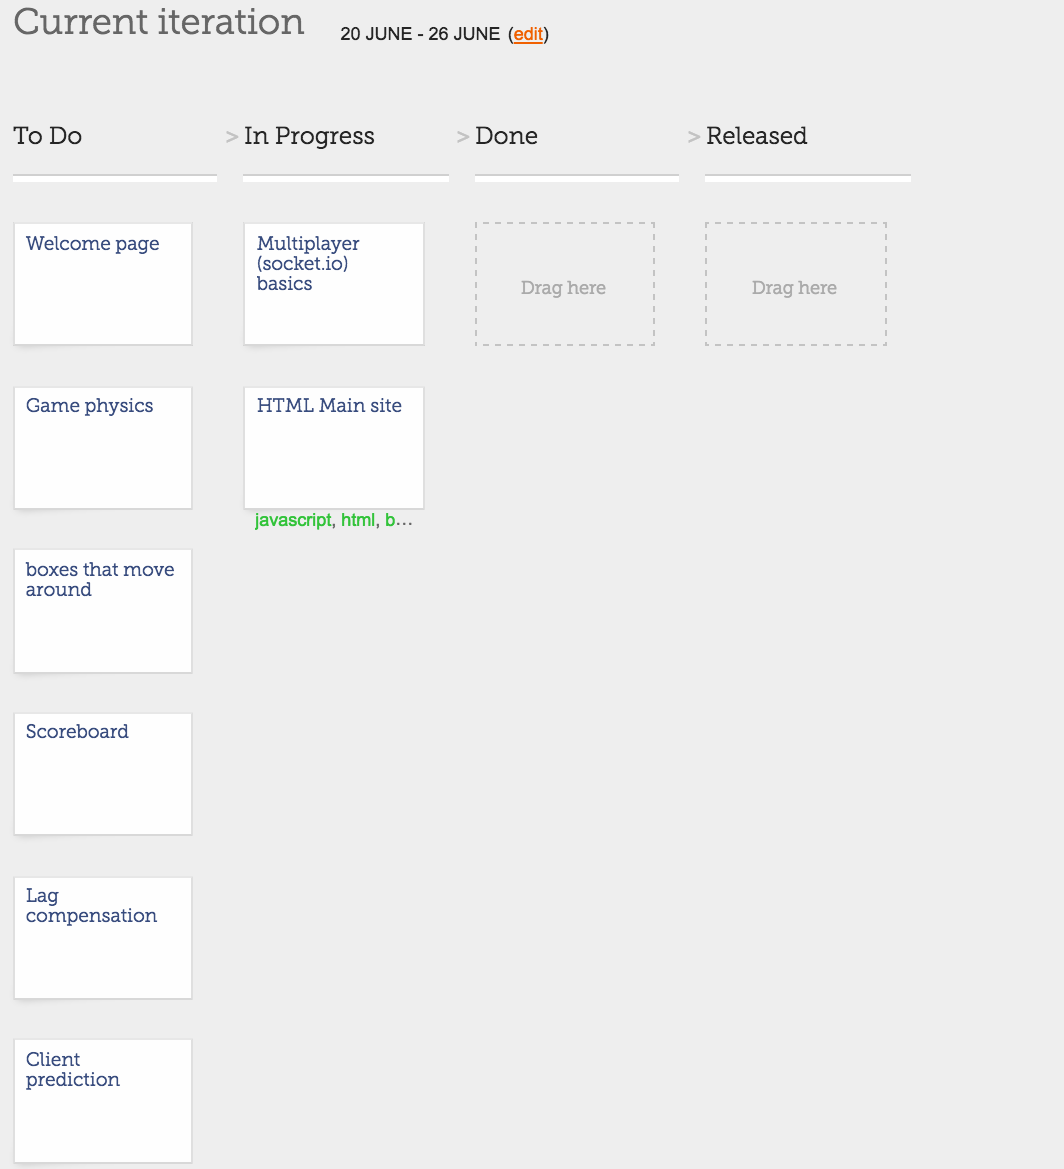
\includegraphics[width=.45\textwidth]{beginning}%
        }%
        \setbox2\hbox{%
                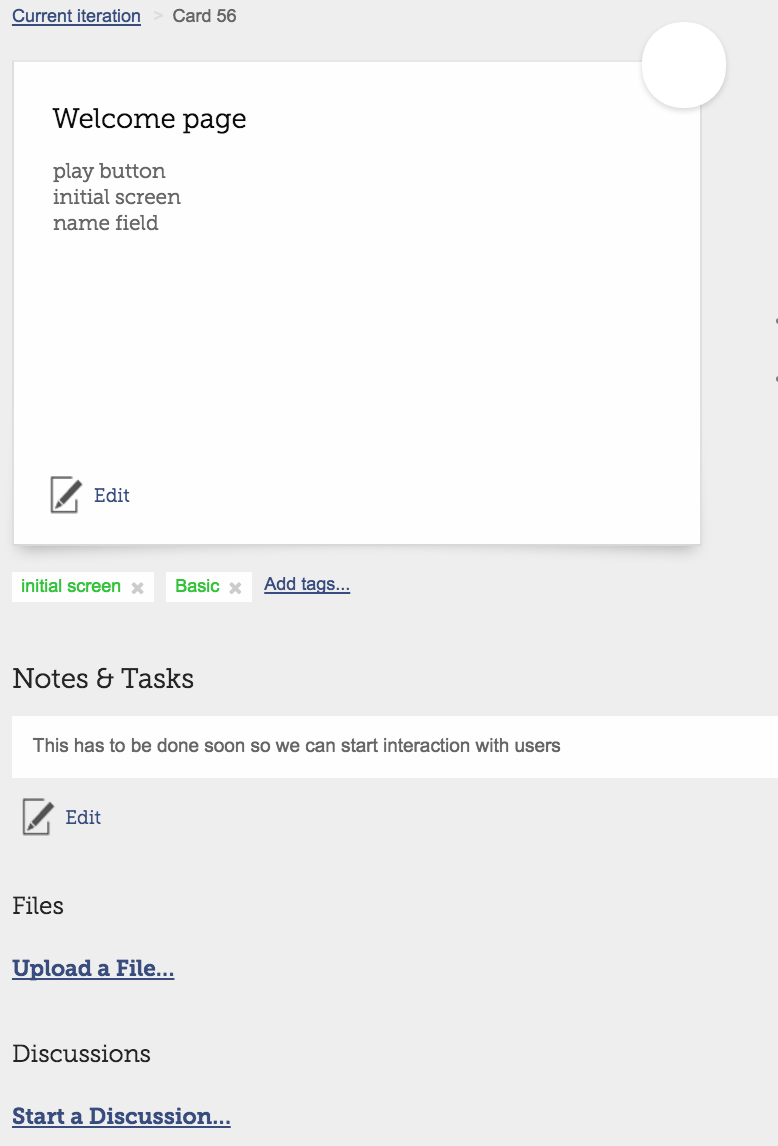
\includegraphics[width=.45\textwidth]{card}%
        }%
        \ifdim\ht0>\ht2
                \setbox0\hbox{%
                        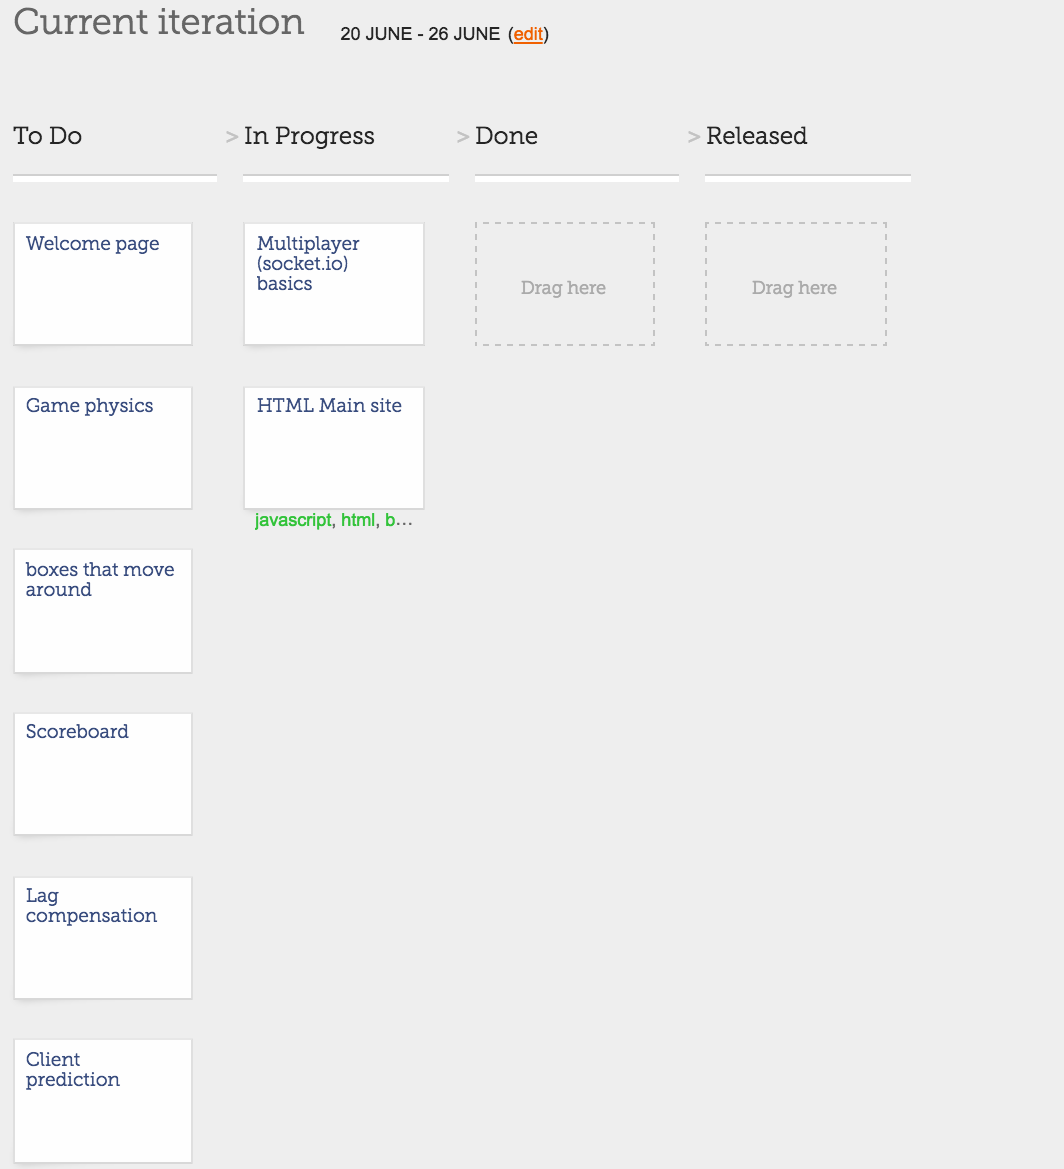
\includegraphics[height=\ht2]{beginning}%
                }%
        \else
                \setbox2\hbox{%
                        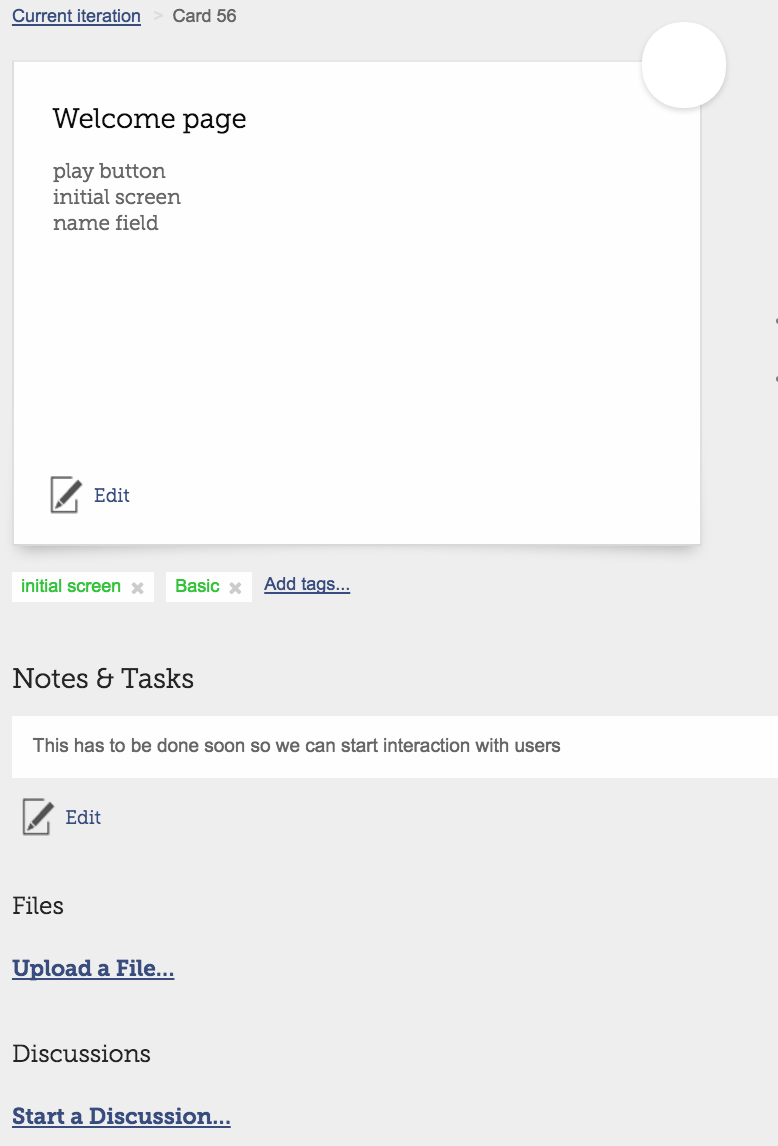
\includegraphics[height=\ht0]{card}%
                }%
        \fi
        \noindent
        \parbox{.45\textwidth}{%
                \centering
                \unhbox0
                \caption{Board at the beginning of the iteration}
                \label{fg:beginning}
        }%
        \hfil
        \parbox{.45\textwidth}{%
                \centering
                \unhbox2
                \caption{A single card and its content}
                \label{fg:card}
        }%
\end{figure}

\begin{figure}[h!]
        \setbox0\hbox{%
                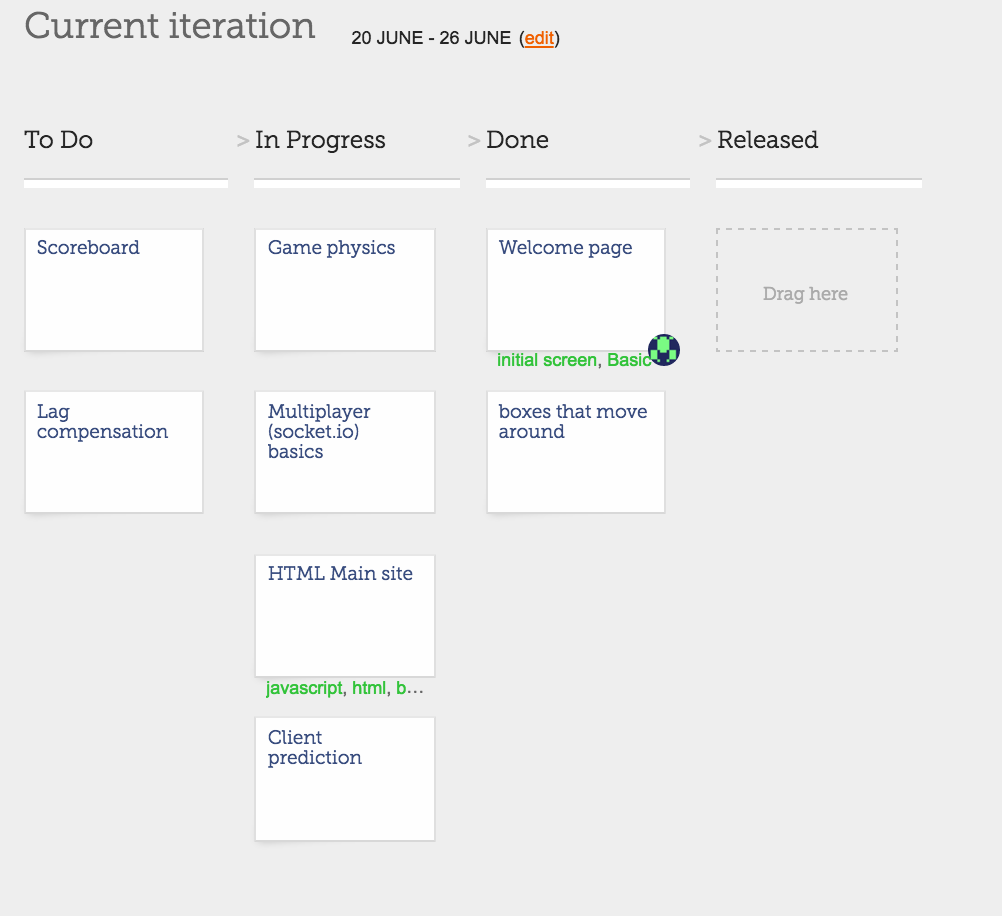
\includegraphics[width=.45\textwidth]{middle}%
        }%
        \setbox2\hbox{%
                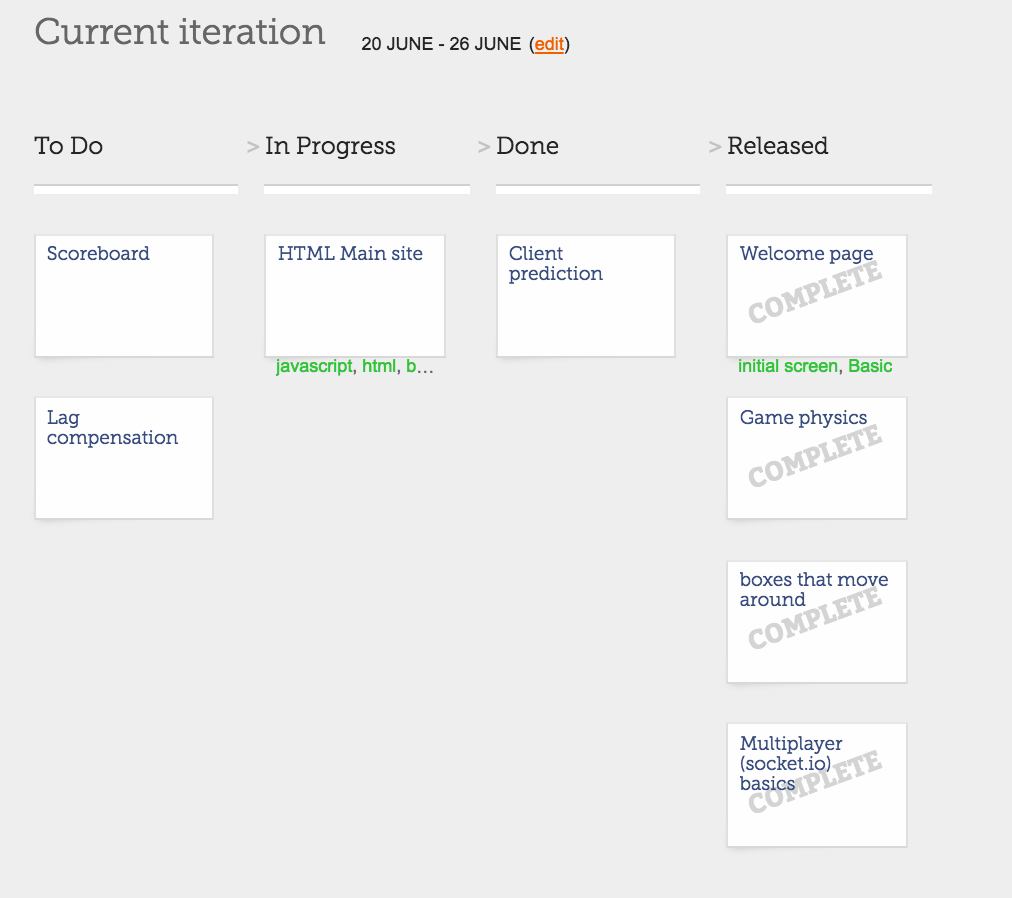
\includegraphics[width=.45\textwidth]{end}%
        }%
        \ifdim\ht0>\ht2
                \setbox0\hbox{%
                        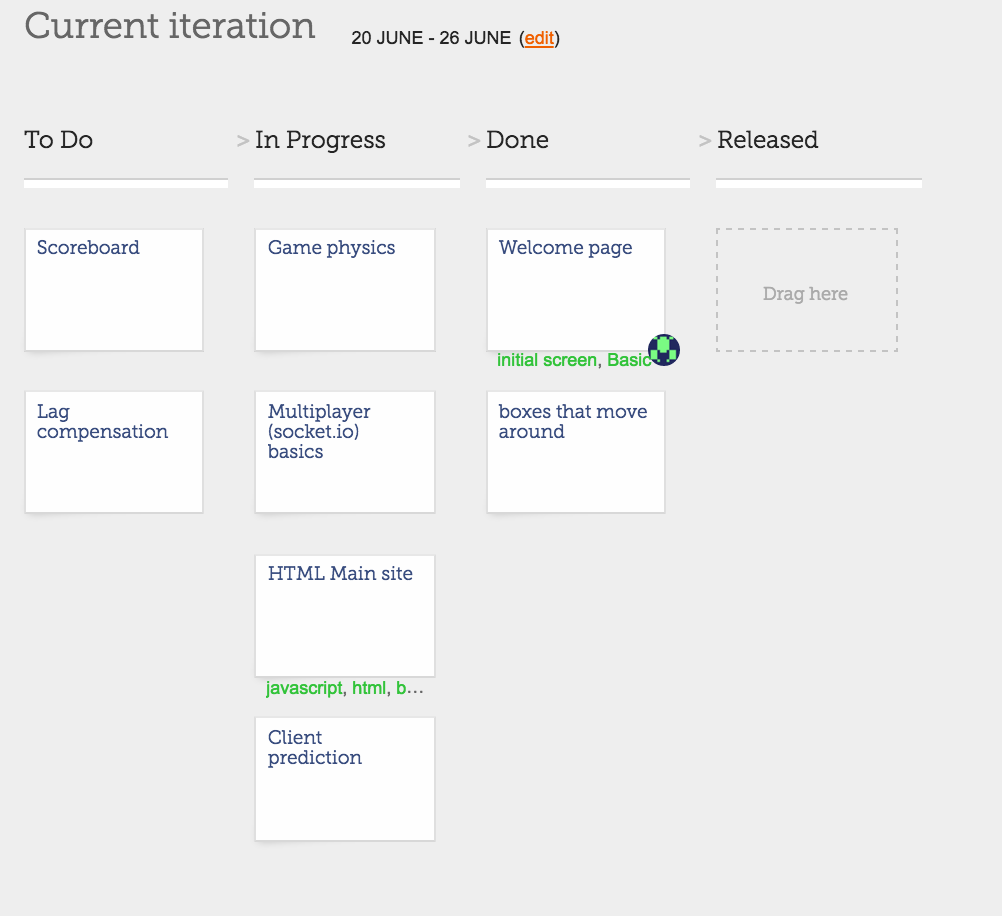
\includegraphics[height=\ht2]{middle}%
                }%
        \else
                \setbox2\hbox{%
                        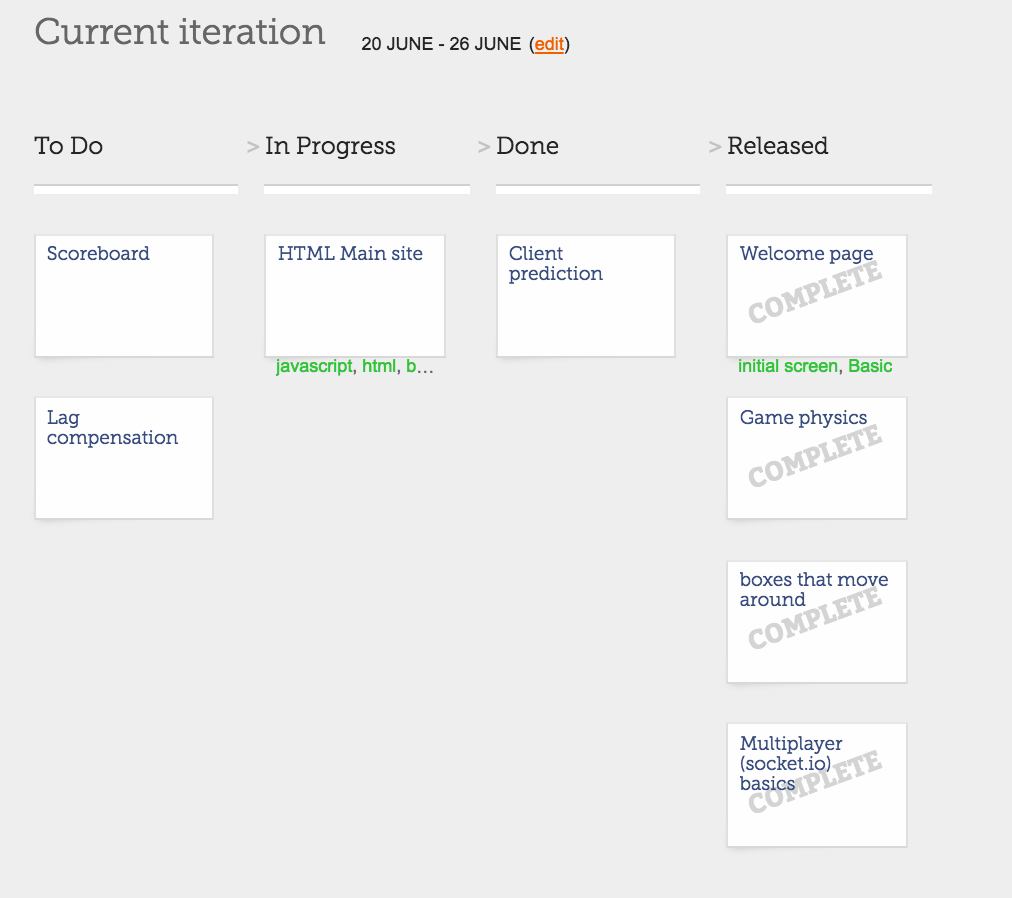
\includegraphics[height=\ht0]{end}%
                }%
        \fi
        \noindent
        \parbox{.45\textwidth}{%
                \centering
                \unhbox0
                \caption{Board at the middle of the iteration}
                \label{fg:middle}
        }%
        \hfil
        \parbox{.45\textwidth}{%
                \centering
                \unhbox2
                \caption{Board at the end of the iteration}
                \label{fg:end}
        }%
\end{figure}

\clearpage
\section{Project Technology}

\textbf{NodeJS} and the \textbf{ExpressJS} framework which is built on top of 
Node allow for incredibly fast server-side development with 
high level javascript constructs and an event driven architecture.
It is the perfect tool for agile web development.

Pure \textbf{Javascript} for the clients gives us complete control over the 
physics and rendering.

\textbf{SocketIO} provides an easy to use WebSocket API for asynchronous
client-server communication.

Finally \textbf{Jquery} for DOM access, hiding and fading parts of the html, 
responding to user input, etc.

\textbf{HTML} and \textbf{CSS} also make up an important part of our frontend.

%----------------------------------------------------------------------------------------

\end{document}
